\section*{Problem statement}
\addcontentsline{toc}{section}{\protect\numberline{}{Problem statement}}

\paragraph{Alignment problem}
% problem statements
We consider the problem of pairwise sequence alignment in the context of genomic
data: given two DNA sequences, one has to be aligned to the other. Two sequences
can be aligned in multiple ways (\cref{fig:alignment-types}). In this thesis we
focus on global and semi-global alignment types only. If both sequences have to
be aligned end to end, we look for a \emph{global alignment} whose minimal
number of edits is known as \emph{edit distance}. If we instead search for an
occurance of a query sequence within a reference sequence, we allow the
alignment to start and end at any reference locations in a \emph{semi-global}
alignment.

% merge
Each sequence from a new biological sample can be compared to a reference genome
(if such is available) in order to identify mutations, quantify expression per
gene, and many other types of analysis. To figure out the location in the
reference each sequence most probably originates from, it should first be
semi-globally aligned to the reference. If the sequences of two proteins or
viruses have been reconstructed, aligning them globally reveals the most
probabale mutations between them.

% alignment types
\begin{figure}[t]  %\begin{floatingfigure}[l]{0.5\textwidth}
    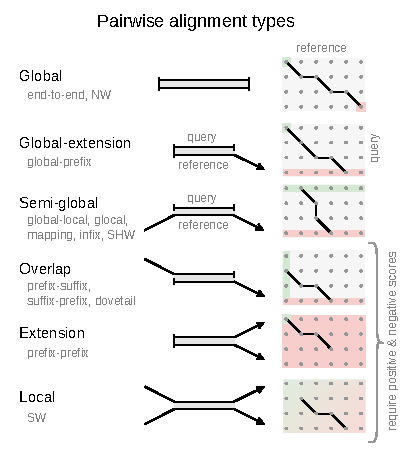
\includegraphics[width=0.5\textwidth]{alignment-types}
	\caption[Alignment types]{Alignment types.}
    \label{fig:alignment-types}
\end{figure}

\paragraph{Optimization metric}
It would have been relatively easy if the alignment would be perfect.
Nevertheless, the real data contains both biological variation and technical
errors resulting from evolution and the sequencing process. A common intuitive
and robust assumption is that an alignment with a minimal number of
single-letter edits (substitutions, insertions and deletions) is the most
plausable explainationo of the divergence of both sequences from an unknown
common ancestor.

\paragraph{Global alignment}

\paragraph{Semi-global alignment}
Formally, we consider the optimal \emph{sequence-to-graph alignment} problem,
the task of finding an optimal base-to-base correspondence between a query
sequence and a (possibly cyclic) walk in the graph. Related alignment problems
have already been formulated as graph shortest path
problems~\cite{jain_complexity_2019}.
 (also called approximate/fuzzy string search outside computational
biology).
We note that in contrast to linear references, reference graphs capture genomic
variation and therefore enable more accurate semi-global
alignments~\citep{garrison_variation_2018}.

Semi-global alignment of reads to a reference genome is an essential and early
step in most bioinformatics pipelines.

Specifically, a \emph{sequence-to-graph} alignment is a base-to-base
correspondence between a given read and a walk in the graph. As sequencing
errors and biological variation result in inexact read alignments, edit distance
is the most common metric that alignment algorithms optimize in order to find
the most probable read origin in the reference. The shortest path approach
naturally fits more complex references than linear, including even graphs with
cycles.

\paragraph{Data}


%\section{Task Description: Alignment to Reference Graphs}
\label{TRIEsec:task}

\paragraph{Scalability and performance}

\paragraph{Guaranteed optimality}

\paragraph{Known limitations}

Quadratic optimal for semi-global

In its general case, it is not solvable for strictly subquadratic time which is
often prohibitively slow. Faster approximate algorithms are instead used in
practice. We employ the \A informed search algorithm in order to design an
optimal algorithm that scales subquadratically for related sequences.